\documentclass[12pt, a4paper, oneside]{ctexart}
\usepackage{amsmath, amsthm, amssymb, bm, graphicx, hyperref, mathrsfs}

\title{\textbf{week5}}
\author{方科晨}
\date{\today}
\linespread{1.5}
\newcounter{problemname}
\newenvironment{problem}{\stepcounter{problemname}\par\noindent\textbf{Problem. }}{\\\par}
\newenvironment{solution}{\par\noindent\textbf{Solution. }}{\\\par}
\newenvironment{note}{\par\noindent\textbf{题目\arabic{problemname}的注记. }}{\\\par}

\begin{document}

\maketitle

\begin{problem} 8
    
    \textbf{(1)} 由于 $A$ 为正定矩阵,故 $\forall x\in \mathbb{R}^n,x^TAx>0$ ,因此,取 $e_i$ 为第 $i$ 维为 $1$ 其余为 $0$ 的向量,有 $e_i^TAe_i=a_{ii}>0$ ,故得证。

    \textbf{(2)} 由于 $a_{11}>0$ ,由上次作业,即本章第 $7$ 题可得 $A_2$ 为对称矩阵。令 $B=\begin{pmatrix}
        a_{11} & a_1^T\\
        0 & A_2
    \end{pmatrix}$ ,则 $b_{ij}=a_{ij}-\frac{a_{1j}*a_{i1}}{a_{11}},\forall i,j\geq 2$ 。对于任意的 $=(x_2,\cdots,x_n)\in\mathbb{R}^{n-1}$ ,有 $$\begin{array}{ll}&\hat{x}^TA_2\hat{x}\\=&\sum_{i=2}^n\sum_{j=2}^n(a_{ij}-\frac{a_{1j}a_{i1}}{a_{11}})x_ix_j\\=&\sum_{i=2}^n\sum_{j=2}^na_{ij}x_ix_j-\sum_{i=2}^n\sum_{j=2}^n\frac{a_{1j}a_{i1}}{a_{11}}x_ix_j-\sum_{i=2}^n\sum_{j=2}^n\frac{a_{1j}a_{i1}}{a_{11}}x_ix_j+\sum_{i=2}^n\sum_{j=2}^n\frac{a_{1j}a_{i1}}{a_{11}}x_ix_j\\=&\sum_{i=2}^n\sum_{j=2}^na_{ij}x_ix_j+\sum_{i=2}^na_{i1}x_ix_1+\sum_{j=2}^na_{1j}x_jx_1+a_{11}x_1x_1\\=&\sum_{i=1}^n\sum_{j=1}^na_{ij}x_ix_j\end{array}$$
    其中 $x_1=-\sum_{j=2}^n\frac{a_{1j}x_j}{a_{11}}=-\sum_{i=2}^n\frac{a_{i1}x_i}{a_{11}}$ ,由于 $A$ 是正定矩阵,所以 $\sum_{i=1}^n\sum_{j=1}^na_{ij}x_ix_j>0$ ,因此 $A_2$ 为正定矩阵。
\end{problem}

\begin{problem} 13

    \begin{figure*}[h!]
        \centering
        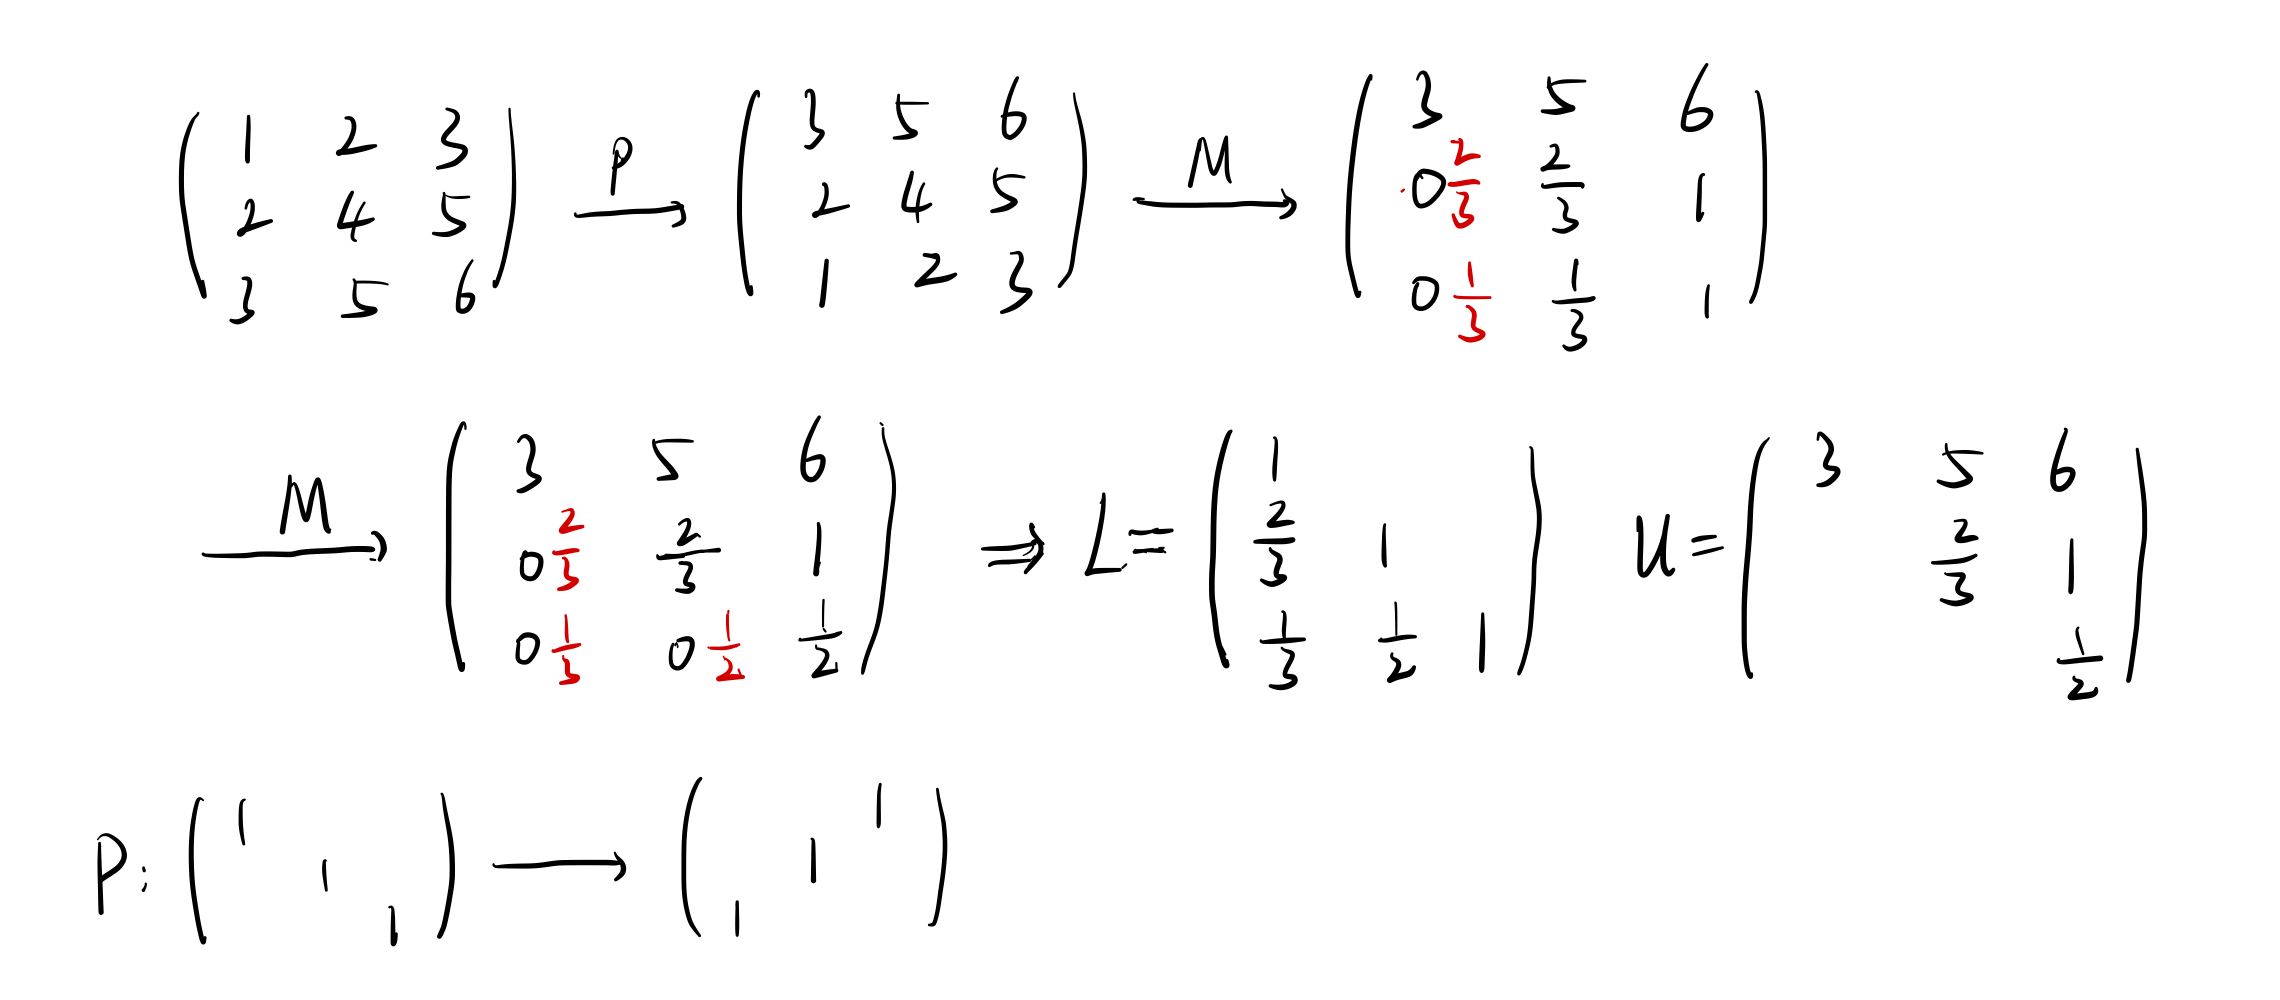
\includegraphics[width=0.95\textwidth]{./pic/pic1.jpeg}
        \caption{A}
    \end{figure*}

    \begin{figure*}[h!]
        \centering
        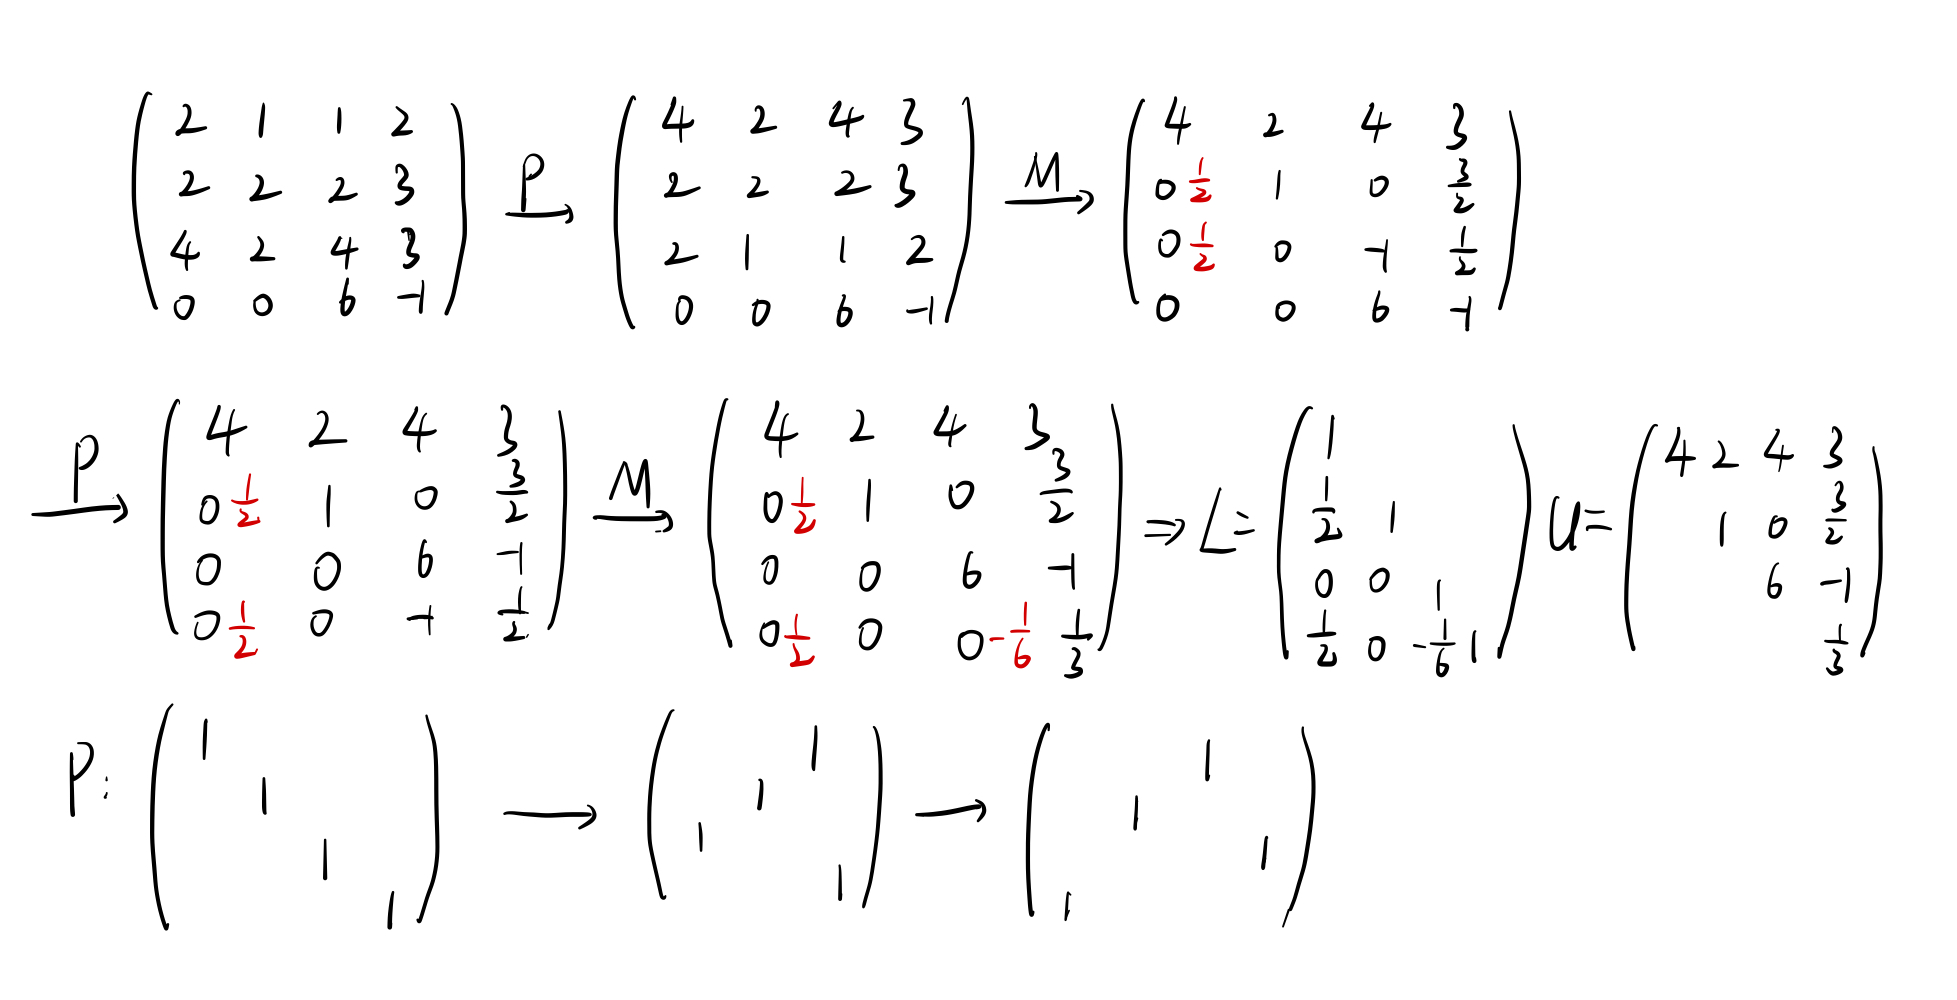
\includegraphics[width=0.95\textwidth]{./pic/pic2.jpeg}
        \caption{B}
    \end{figure*}
    如图
\end{problem}

\begin{problem} 14
    
    先使用部分主元分解求得 $PB=LU,QC=RS$ ,然后原式 $x=B^{-1}(2A+I)(C^{-1}+A)b=U^{-1}L^{-1}P(2A+I)(S^{-1}R^{-1}Qb+Ab)$ 。从右往左看, $Ab$ 直接计算可得, $Qb$ 也直接计算可得,由于 $R$ 为下三角阵,故求 $R^{-1}(QB)$ 从上往下求解便可,求解完后 $S^{-1}(R^{-1}Qb)$ 同理,然后两个向量相加,与 $(2A+I)$ 直接相乘,再与 $P$ 相乘,然后与 $L^{-1}$ 和 $U^{-1}$ 相乘时同理从上往下或从下往上求解便可。
\end{problem}

\begin{problem} 15
    
    \begin{figure*}[h!]
        \centering
        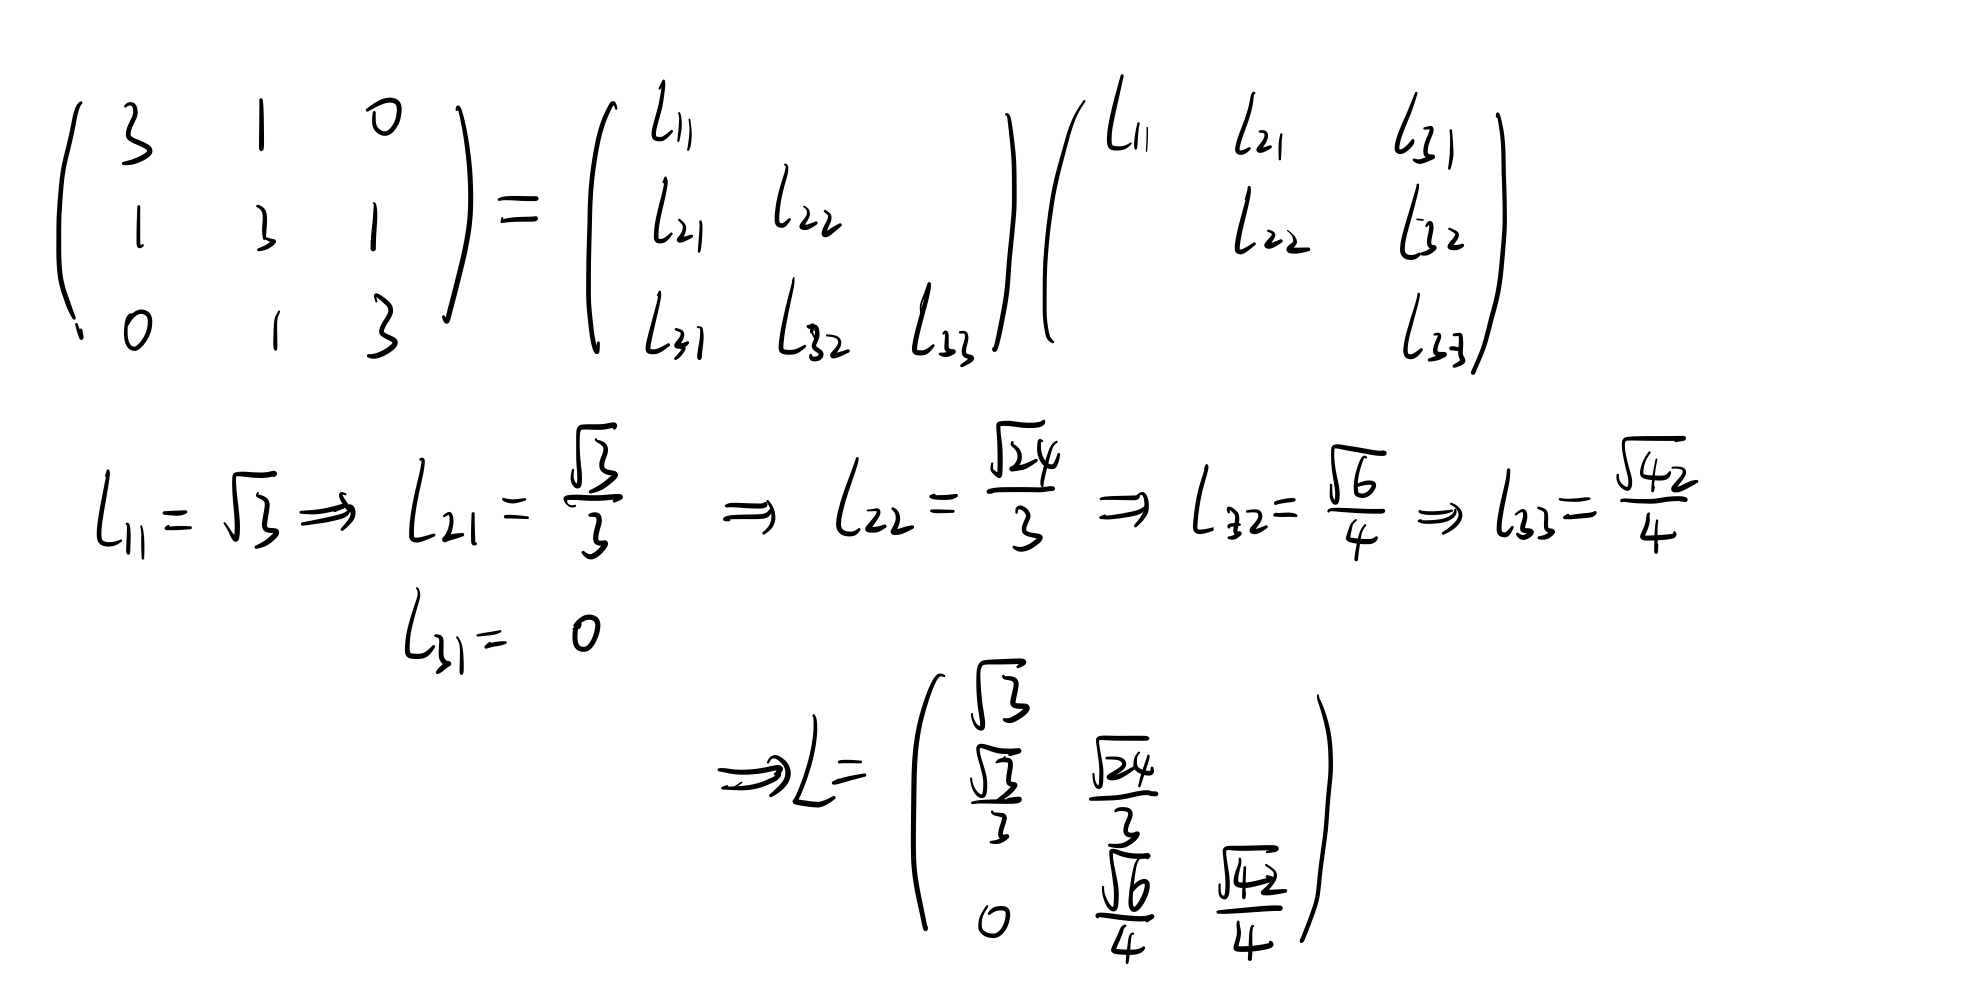
\includegraphics[width=0.95\textwidth]{./pic/pic3.jpeg}
        \caption{A}
    \end{figure*}
    \begin{figure*}[h!]
        \centering
        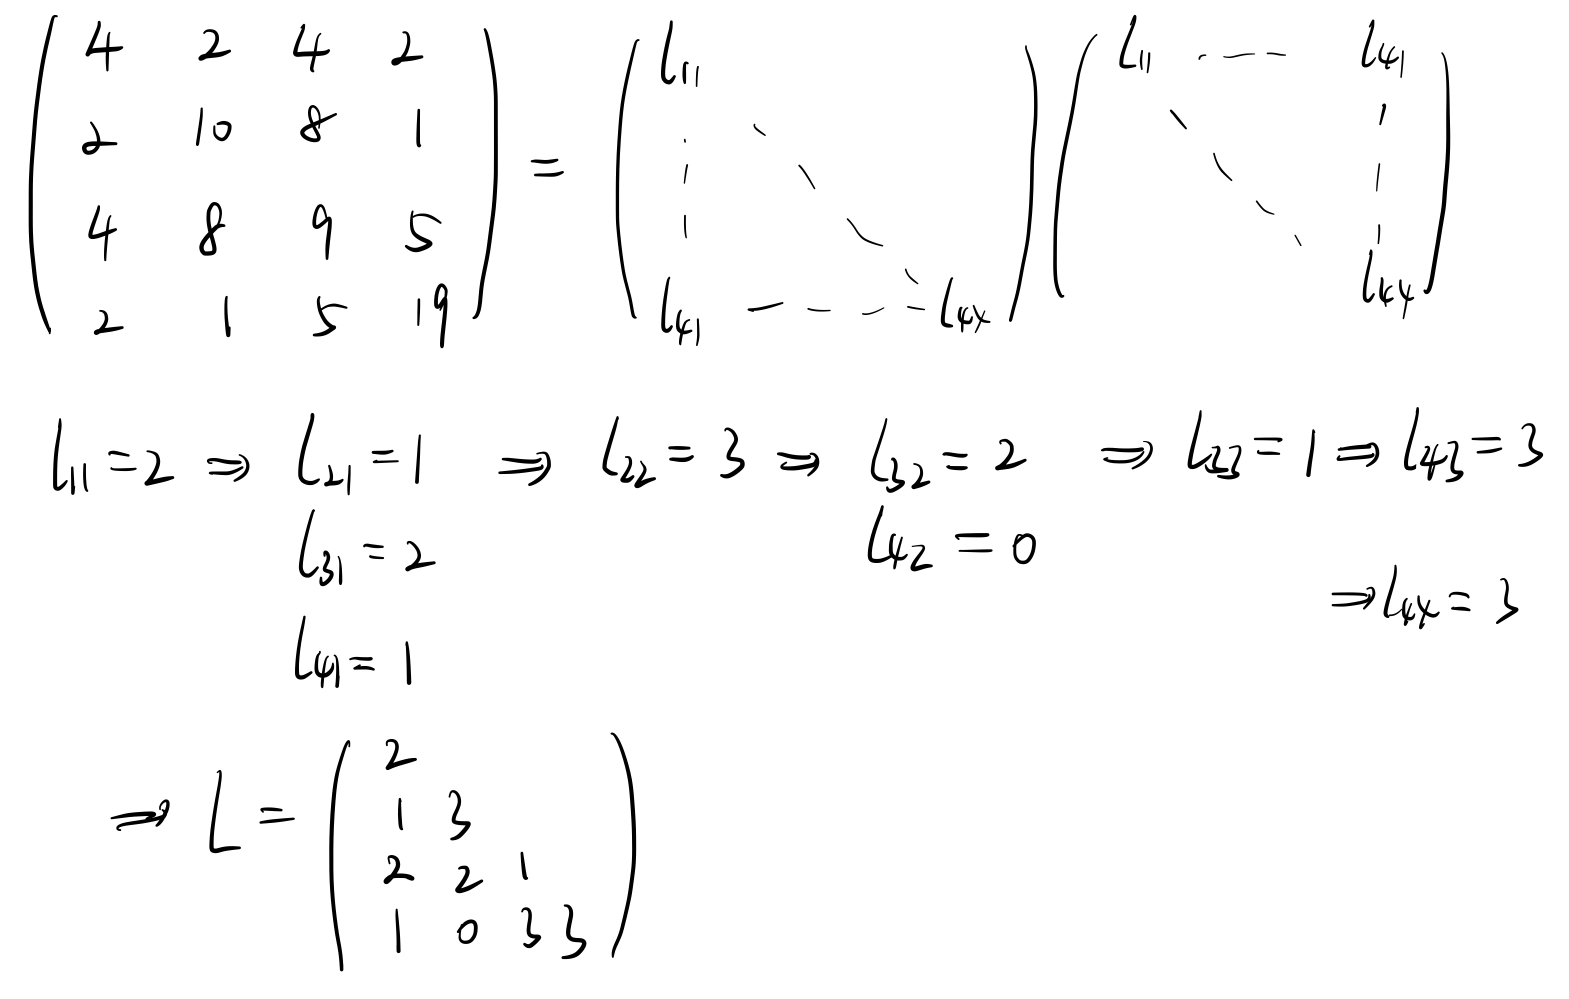
\includegraphics[width=0.95\textwidth]{./pic/pic4.jpeg}
        \caption{B}
    \end{figure*}
    如图
\end{problem}

\begin{problem} 16
    
    \begin{figure*}[h!]
        \centering
        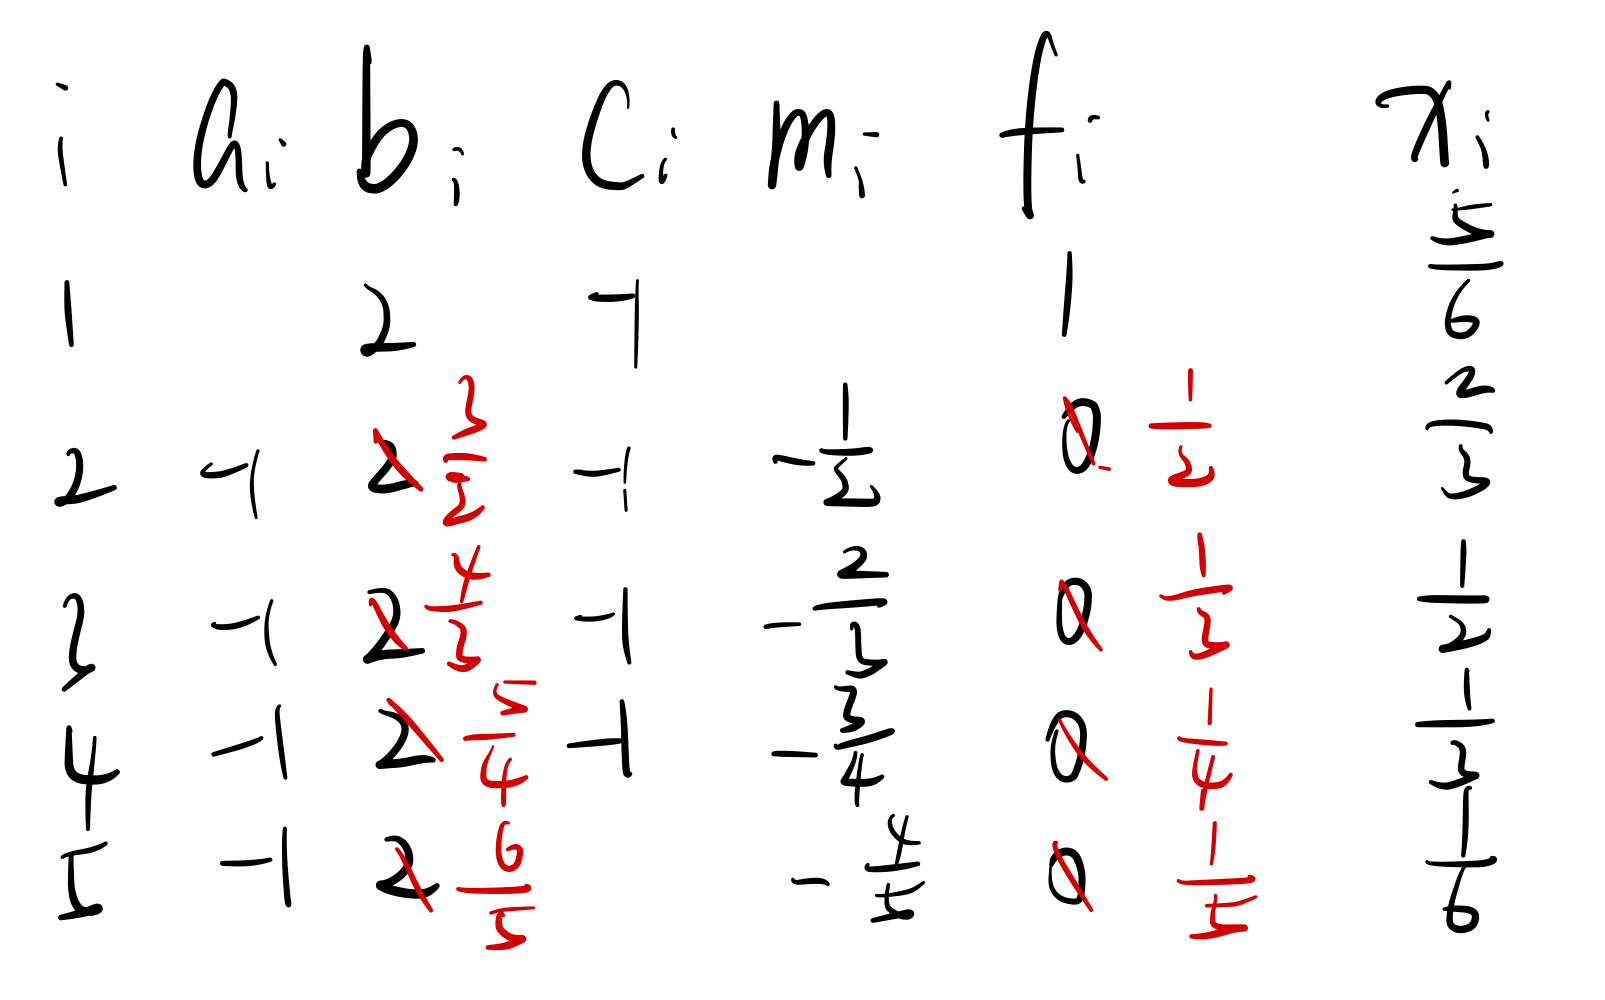
\includegraphics[width=0.95\textwidth]{./pic/pic5.jpeg}
    \end{figure*}
    如图
\end{problem}

\begin{problem} 18(1)
    
    $A$ 按列严格对角占优,即 $|a_{jj}|>\sum_{i=1,i\neq j}^n |a_{ij}|$

    不妨加强结论,证明对每一个主元做完所有的消元过程后,即从 $A$ 消元成 $B=A^{(2)}=\begin{pmatrix}
        a_{11} & a_1^T\\
        0 & A_2
    \end{pmatrix}$ ,我们有 $A_2$ 仍然是列严格对角占优。那么原命题就显然成立。\\

    由消元过程可得, $b_{ij}=a_{ij}-\frac{a_{1j}*a_{i1}}{a_{11}},\forall i,j\geq 2$ ,需要证明 $|b_{ii}|>\sum_{j=2,j\neq i}^n |b_{ij}|, \forall i\geq 2$ 。我们有如下推导:
    $$\begin{array}{lll}
        & |b_{ii}|-\sum_{j=2,j\neq i}^n |b_{ij}|\\
        =&|a_{ii}-\frac{a_{1i}a_{i1}}{a_{11}}|-\sum_{j=2,j\neq i}^n|a_{ij}-\frac{a_{1j}a_{i1}}{a_{11}}|\\
        \geq&|a_{ii}|-|\frac{a_{1i}a_{i1}}{a_{11}}|-\sum_{j=2,j\neq i}^n(|a_{ij}|+|\frac{a_{1j}a_{i1}}{a_{11}}|)&\textrm{(第一个列严格对角占优,第二个绝对值不等式)}\\
        =&|a_{ii}|-\sum_{j=2,j\neq i}^n|a_{ij}|-\sum_{j=2}^n |\frac{a_{1j}a_{i1}}{a_{11}}|\\
        =&|a_{ii}|-\sum_{j=2,j\neq i}^n|a_{ij}|- |a_{i1}|\frac{\sum_{j=2}^n |a_{1j}|}{|a_{11}|}\\
        >&|a_{ii}|-\sum_{j=2,j\neq i}^n|a_{ij}|- |a_{i1}|&\textrm{(由列严格对角占优)}\\
        =&|a_{ii}|-\sum_{j=1,j\neq i}^n|a_{ij}|\\
        >&0
    \end{array}$$

    故加强命题得证,故原命题得证。
    % 不妨加强结论,证明 $|a_{ii}^{(k)}|>\sum_{s=1,s\neq i}^n|a_{si}^{(k)}|=\sum_{s=k,s\neq i}^n|a_{si}^{(k)}|$
    % 归纳法,假设前 $k-1$ 步都满足 $|a_{ii}^{(j)}|>\sum_{s=j}^n|a_{si}^{(j)}|,j=1,\cdots,k-1,i\geq j$ 。
    % 由消元过程有 $a_{js}^{(k)}=a_{js}-\sum_{i=1}^{k-1} a_{is}^{(i)}\cdot \frac{a_{ji}^{(i)}}{a_{ii}^{(i)}}$ 。
    % 我们有 $$\begin{array}{ll}&|a_{ss}^{(k)}|-\sum_{j=k,j\neq s}^n|a_{js}^{(k)}|\\
    % =&|a_{ss}-\sum_{i=1}^{k-1}a_{is}^{(i)}\frac{a_{si}^{(i)}}{a_{ii}^{(i)}}|-\sum_{j=k,j\neq s}^n|a_{js}-\sum_{i=1}^{k-1} |a_{is}^{(i)}\cdot \frac{a_{ji}^{(i)}}{a_{ii}^{(i)}}|\\
    % >&|a_{ss}|-|\sum_{i=1}^{k-1}a_{is}^{(i)}\frac{a_{si}^{(i)}}{a_{ii}^{(i)}}|-\sum_{j=k,j\neq s}^n(|a_{js}|+\sum_{i=1}^{k-1} |a_{is}^{(i)}\cdot \frac{a_{ji}^{(i)}}{a_{ii}^{(i)}}|)\\
    % >&(|a_{ss}|-\sum_{j=k,j\neq s}^n|a_{js}|)-\sum_{j=k}^n\sum_{i=1}^{k-1} |a_{is}^{(i)}\cdot \frac{a_{ji}^{(i)}}{a_{ii}^{(i)}}|\\
    % =&(|a_{ss}|-\sum_{j=k,j\neq s}^n|a_{js}|)-\sum_{i=1}^{k-1}|a_{is}^{(i)}| (\sum_{j=k}^n |\frac{a_{ji}^{(i)}}{a_{ii}^{(i)}}|)\\
    % =&(|a_{ss}|-\sum_{j=k,j\neq s}^n|a_{js}|)-\sum_{i=1}^{k-1}|a_{is}^{(i)}|  \frac{\sum_{j=k}^n|a_{ji}^{(i)}|}{|a_{ii}^{(i)}|}\\
    % >&(|a_{ss}|-\sum_{j=k,j\neq s}^n|a_{js}|)-\sum_{i=1}^{k-1}|a_{is}^{(i)}|  \frac{|a_{ii}^{(i)}|}{|a_{ii}^{(i)}|}\\
    % =&(|a_{ss}|-\sum_{j=k,j\neq s}^n|a_{js}|)-\sum_{i=1}^{k-1}|a_{is}^{(i)}|  \\
    % \end{array}
    % $$
    % 又因为前 $k-1$ 次都不需要交换主元,可得 $|a_{si}|\leq|a_{ii}|$ 。因此有 $|\sum_{i=1}^{k-1} a_{ik}\cdot \frac{a_{si}}{a_{ii}}| \leq \sum_{i=1}^{k-1}|a_{ik}|\cdot |\frac{a_{ki}}{a_{ii}}| \leq \sum_{i=1}^{k-1}|a_{ik}|$ 。因此 $|a_{kk}^{(k)}|$
\end{problem}

\end{document}
